%% monografia.tex, fabiokepler, jeancheiran
%% Copyright 2012-2018 by UNIPAMPA LaTeX group at https://bitbucket.org/  unipampaalegrete/monografias-cc-es-repo/
%%
%% This work may be distributed and/or modified under the conditions of the LaTeX Project Public
%% License, either version 1.3 of this license or (at your option) any later version.
%% The latest version of this license is in
%%   http://www.latex-project.org/lppl.txt
%% and version 1.3 or later is part of all distributions of LaTeX version 2005/12/01 or later.
%%
%% Based on the example file abtex2-modelo-trabalho-academico.tex of the abntex2 package
%% (http://abntex2.googlecode.com/) and on the ppgccufmg 1.45beta2 class
%% (http://vilarneto.com/ppgccufmg,
%% http://www.dcc.ufmg.br/pos/alunos/modelodisstese.php
%% and http://www.dcc.ufmg.br/~mirella).
%%
%% Adapted for the Computer Science program at UNIPAMPA (http://www.unipampa.edu.br)
%% by Fabio Kepler (fabio@kepler.pro.br) and Jean Cheiran (jeancheiran@unipampa.edu.br).
%%
%% Version 2.5 - 2018/08
%% Version 2.4 - 2017/05
%% Version 2.3 - 2013/03

% +++++++++++++++++++++++++++++++++++++++++++++++++++++++++++++++++++++++++++++++++++++++++++++++++
% Este modelo utiliza o pacote abnTeX2. Veja como instalá-lo em seu ambiente em
% http://abntex2.googlecode.com/.
% -------------------------------------------------------------------------------------------------
% abnTeX2: Modelo de Trabalho Acadêmico (tese de doutorado, dissertação de
% mestrado e trabalhos monográficos em geral) em conformidade com
% ABNT NBR 14724:2011: Informação e documentação - Trabalhos acadêmicos -
% Apresentação
% -------------------------------------------------------------------------------------------------
% Normas institucionais utilizadas:
% http://porteiras.r.unipampa.edu.br/portais/sisbi/programa-de-capacitacao/
% +++++++++++++++++++++++++++++++++++++++++++++++++++++++++++++++++++++++++++++++++++++++++++++++++

\documentclass[12pt,openright,twoside,a4paper,chapter=TITLE]{abntex2}    % frente e verso
%\documentclass[12pt,oneside,a4paper]{abntex2}            % apenas frente

% +++++++++++++++++++++++++++++++++++++++++++++++++++++++++++++++++++++++++++++++++++++++++++++++++
% PACOTES
% -------------------------------------------------------------------------------------------------
% Pacotes fundamentais
\usepackage{cmap}           % Mapeamento de caracteres especiais no PDF
\usepackage{lmodern}        % Usa fonte Latin Modern
\usepackage[T1]{fontenc}    % Seleção de codificação de fonte
\usepackage[utf8]{inputenc} % Codificação do arquivo (conversão automática dos acentos)
\usepackage[brazil]{babel}  % Idioma para hifenização e tradução de vários elementos
\usepackage{makeidx}        % Criação de índice
\usepackage{hyperref}       % Formatação do índice
\usepackage{lastpage}       % Usado pela Ficha catalográfica
\usepackage{indentfirst}    % Indenta o primeiro parágrafo de cada seção
\usepackage[usenames,dvipsnames]{xcolor}  % Controle das cores (com nomes)
\usepackage{graphicx}       % Inclusão de gráficos
\usepackage{booktabs}       % Formatação de tabelas
% -------------------------------------------------------------------------------------------------
% Para citações
\usepackage[brazilian,hyperpageref]{backref} % Páginas com as citações na bibliografia
\usepackage[alf,abnt-emphasize=bf]{abntex2cite} % Citações padrão ABNT (alfanumérico)
% -------------------------------------------------------------------------------------------------
% Pacotes opcionais
\usepackage{nomencl}        % Para criar uma lista de símbolos
\usepackage{acro}           % Para usar acrônimos e abreviaturas
\usepackage{tikz}           % Para fazer figuras, diagramas e gráficos integrados e elegantes
\usepackage{pgfplots}       % Usa o pacote tikz para fazer gráficos muito melhores que os do Excel
\usepackage{pgfplotstable}  % Para gerar tabelas automaticamente a partir de arquivos com dados
\usepackage{filecontents}   % Para colocar o conteúdo de um arquivo dentro de um arquivo tex
\usepackage{todonotes}      % Para criar anotações durante o desenvolvimento do texto
%\usepackage{multirow}       % Permite fazer tabelas com múltiplas linhas
\let\newfloat=\undefined    % Workaround para usar o pacote algorithm
%\usepackage{algorithm}      % Para escrever algoritmos
%\usepackage{clrscode}       % Para escrever algoritmos
%\usepackage{clrscode3e}     % Para escrever algoritmos; mais simples que os pacotes acima
\usepackage{pdfpages}        % Para incluir a folha de aprovação assinada em PDF

%----
% marcar a data
\usepackage{fancyhdr}
\usepackage[us,12hr]{datetime} % `us' makes \today behave as usual in TeX/LaTeX
\fancypagestyle{plain}{
\fancyhf{}
%\rfoot{Compiled on {\ddmmyyyydate\today} at \currenttime}
\lfoot{Page \thepage}
\renewcommand{\headrulewidth}{0pt}}
\pagestyle{plain}


%-------------------------------------------------------------------------------------------------
% meus pacotes
\usepackage{breakcites}
\usepackage{algorithm}
\usepackage[noend]{algpseudocode}
\usepackage{multirow}
\usepackage{fancyvrb}
\usepackage{xspace}
\usepackage{color}
\usepackage{longtable}
\usepackage[hide]{chato-notes}
\usepackage{amssymb}% http://ctan.org/pkg/amssymb
\usepackage{pifont}% http://ctan.org/pkg/pifont
\newcommand{\cmark}{\ding{51}}%
\newcommand{\xmark}{\ding{55}}%
\usepackage[]{appendix}%

% -------------------------------------------------------------------------------------------------
% Configurações de pacotes
% -------------------------------------------------------------------------------------------------
\addto\captionsbrazil{
  \renewcommand{\listfigurename}{Lista de figuras}
}
% -------------------------------------------------------------------------------------------------
% Configurações do pacote backref
% Usado sem a opção hyperpageref de backref
\renewcommand{\backrefpagesname}{Citado na(s) página(s):~}
% Texto padrão antes do número das páginas
\renewcommand{\backref}{}
% Define os textos da citação
\renewcommand*{\backrefalt}[4]{
    \ifcase #1 %
        Nenhuma citação no texto.%
    \or
        Citado na página #2.%
    \else
        Citado #1 vezes nas páginas #2.%
    \fi}%
    
\newcommand{\standalone}[0]{\textit{standalone}\xspace}
% -------------------------------------------------------------------------------------------------
% Configurações de aparência do PDF final
%\definecolor{blue}{RGB}{41,5,195}
% \definecolor{webgreen}{rgb}{0,.5,0}
% Metainformações do PDF e cores dos links
\hypersetup{
  portuguese,
  %backref=true,
  %pagebackref=true,
  %bookmarks=true,             % show bookmarks bar?
  %bookmarksnumbered=true,
  bookmarksdepth=4,
  pdftitle={\@title},
  pdfauthor={\@author},
  pdfsubject={\imprimirpreambulo},
  pdfkeywords={UNIPAMPA}{Computação}{UNIPAMPA}{abntex}{TCC},
  %pdfproducer={LaTeX with abnTeX2},     % producer of the document
  pdfcreator={\@author},
  colorlinks=true,           % false: boxed links; true: colored links
  linkcolor=black,            % color of internal links
  citecolor=black,            % color of links to bibliography
  filecolor=black,         % color of file links
  urlcolor=black
}
%   linktocpage,
%   colorlinks,
%   citecolor=webgreen,
%   urlcolor=Maroon,
%   linkcolor=RoyalBlue,
%   filecolor=black,
% -------------------------------------------------------------------------------------------------
% Espaçamentos entre linhas e parágrafos
% O tamanho do parágrafo é dado por
\setlength{\parindent}{1.3cm}
% Controle do espaçamento entre um parágrafo e outro
\setlength{\parskip}{0.2cm} % tente também \onelineskip
% Controles do espaçamento entre linhas
%\OnehalfSpacing       % espaçamento um e meio (padrão);
%\DoubleSpacing        % espaçamento duplo
%\SingleSpacing        % espaçamento simples
% -------------------------------------------------------------------------------------------------
% Para o pacote de acrônimos
\acsetup{hyperref=true,index=true} %first-style=short}
% -------------------------------------------------------------------------------------------------
% Para o pacote tikz, pgfplots e pgfplotstable
\usetikzlibrary{arrows,chains,matrix,positioning,decorations.pathreplacing,calc}
% -------------------------------------------------------------------------------------------------
% Para poder usar subfiguras e subtabelas
\newsubfloat{figure}
\newsubfloat{table}
\providecommand*{\subfigureautorefname}{\figureautorefname}
% +++++++++++++++++++++++++++++++++++++++++++++++++++++++++++++++++++++++++++++++++++++++++++++++++

%===========================================================
% REVIEW COMMANDS
\newcommand{\missingcite}[1]{\textcolor{red}{[FALTA REF ou é BOM USAR UMA REF] #1}} % when you don't have the reference
\newcommand{\missingexamples}[1]{\textcolor{red}{[FALTA EXEMPLO] #1}} % when you don't have the reference
\newcommand{\missingthings}[1]{\textcolor{red}{[FALTA CONTEUDO] #1}} % when you don't have the reference


\newcommand{\blue}[1]{\textcolor{black}{#1}} % blue: improved writing
\newcommand{\purple}[1]{\textcolor{black}{#1}} % purple: answering reviews' comments
\newcommand{\red}[1]{\textcolor{black}{#1}} % red: hard to understand 
\newcommand{\magenta}[1]{\textcolor{black}{#1}} %magenta: needs to be checked (e.g. references, writing, etc.)

\newcommand{\gray}[1]{\textcolor{gray}{#1}} % proposed
\newcommand{\writingissue}[1]{\textcolor{red}{[WRITING ISSUE?] #1}} % to be removed
\newcommand{\DK}[1]{\textcolor{orange}{DK: #1}} % Kreutz
\newcommand{\omite}[1]{}

\newcommand{\covid}[1]{COVID-19}



% +++++++++++++++++++++++++++++++++++++++++++++++++++++++++++++++++++++++++++++++++++++++++++++++++
% Informações de dados para CAPA e FOLHA DE ROSTO
% -------------------------------------------------------------------------------------------------
\titulo{Modelo preditivo para prognóstico de pacientes com COVID-19}
\autor{Gustavo Cardozo Rodrigues}
\local{Alegrete}
\data{2021}
\orientador{Prof. Dr. Diego Kreutz}
\coorientador{Prof. Dr. Mirkos Ortiz Martins} % Se houver
\instituicao{Universidade Federal do Pampa}
%\tipotrabalho{Projeto de Trabalho de Conclusão de Curso~} % Para TCC I
\tipotrabalho{Trabalho de Conclusão de Curso~} % Para TCC II
% O preambulo deve conter o tipo do trabalho, o objetivo, o nome da instituição e a área de concentração
\preambulo{\imprimirtipotrabalho apresentado ao Curso de Graduação em Ciência da
           Computação da Universidade Federal do Pampa como requisito parcial para a obtenção do
           título de Bacharel em Ciência da Computação.}
% +++++++++++++++++++++++++++++++++++++++++++++++++++++++++++++++++++++++++++++++++++++++++++++++++

% -------------------------------------------------------------------------------------------------
% Compila o indice
\makeindex
% Compila a lista de abreviaturas e siglas
% Para funcionar, o seguinte comando deve ser executado:
% makeindex ARQUIVO_PRINCIPAL.nlo -s nomencl.ist -o ARQUIVO_PRINCIPAL.nls
\makenomenclature
% -------------------------------------------------------------------------------------------------

% -------------------------------------------------------------------------------------------------
% Abreviaturas (definido pelo parâmetro 'class')
\DeclareAcronym{fig}{
  short = Fig.,
  long  = Figura,
  class = abreviaturas
}
% -------------------------------------------------------------------------------------------------
% Acrônimos/Siglas (definido pelo parâmetro 'class')
\DeclareAcronym{tcc}{
  short = TCC,
  long  = Trabalho de Conclusão de Curso,
  long-plural-form = Trabalhos de Conclusão de Curso,
  class = acronimos
}
% -------------------------------------------------------------------------------------------------
% Nomenclaturas/Símbolos
\nomenclature{$A_i$}{Área do $i^{esimo}$ componente}
\nomenclature{456}{Isto é um número}
\nomenclature{123}{Isto é outro número}
\nomenclature{$n$}{Tamanho da entrada}
\nomenclature{$V$}{Vetor de elementos}
\nomenclature{$\mathcal{T}$}{Conjunto de trabalhos de TCC}

% -------------------------------------------------------------------------------------------------
% Inclui alguns ajustes finos para que fique de acordo com o Manual de Normatização
% Pequenos consertos e ajustes para que fique de acordo com o Manual de Normatização 2011.

\setlength{\ABNTEXsignwidth}{12cm}

% ---
% Impressão da Capa
\renewcommand{\imprimircapa}{%
  \begin{capa}%
    \center
    {\ABNTEXchapterfont\large\MakeUppercase\imprimirinstituicao}
    
    \vspace*{\fill}
    {\ABNTEXchapterfont\large\imprimirautor}

    \vspace*{\fill}
    {\ABNTEXchapterfont\bfseries\LARGE\imprimirtitulo}
    \vspace*{\fill}
    ~
    \vspace*{\fill}

    {\large\imprimirlocal}
    \par
    {\large\imprimirdata}

    \vspace*{1cm}
  \end{capa}
}
% ---


% ---
% Impressão da Folha de Rosto
\makeatletter
\renewcommand{\folhaderostocontent}{
  \begin{center}

    {\ABNTEXchapterfont\large\imprimirautor}

    \vspace*{\fill}%\vspace*{\fill}
    {\ABNTEXchapterfont\bfseries\Large\imprimirtitulo}
    \vspace*{\fill}

    \abntex@ifnotempty{\imprimirpreambulo}{%
      \hspace{.45\textwidth}
      \begin{minipage}{.5\textwidth}
        {\SingleSpacing
        \imprimirpreambulo}

        \vspace*{1em}
        \imprimirorientadorRotulo~\imprimirorientador\par

        \abntex@ifnotempty{\imprimircoorientador}{%
          \vspace*{1em}
          \imprimircoorientadorRotulo~\imprimircoorientador%
        }%

      \end{minipage}%
      \vspace*{\fill}
    }%

    {\large\imprimirlocal}
    \par
    {\large\imprimirdata}
    \vspace*{1cm}

  \end{center}
}
\makeatother
% ---

% ---
\renewcommand{\ABNTEXchapterfont}{\rmfamily\bfseries}
\setsecheadstyle{\rmfamily\bfseries}

\renewcommand{\ABNTEXchapterfontsize}{\normalsize}
\renewcommand{\ABNTEXsectionfontsize}{\normalsize}
\renewcommand{\ABNTEXsubsectionfontsize}{\normalsize}
\renewcommand{\ABNTEXsubsubsectionfontsize}{\normalsize}
\renewcommand{\ABNTEXsubsubsubsectionfontsize}{\normalsize}

% Espaçamento entre título e texto
\setlength\afterchapskip{\lineskip}

% Espaçamento entre parágrafos
\setlength{\parskip}{0.cm}

% ---




% *************************************************************************************************
\begin{document}
% *************************************************************************************************

% +++++++++++++++++++++++++++++++++++++++++++++++++++++++++++++++++++++++++++++++++++++++++++++++++
% ELEMENTOS PRÉ-TEXTUAIS
% +++++++++++++++++++++++++++++++++++++++++++++++++++++++++++++++++++++++++++++++++++++++++++++++++
% \pretextual

% -----------------------------------------------
% Capa [OBRIGATÓRIO]
% -----------------------------------------------
%Compiled on {\ddmmyyyydate\today} at \currenttime
\imprimircapa
% -----------------------------------------------
% Folha de rosto [OBRIGATÓRIO]
% -----------------------------------------------
% (ver documentação do abntex2 caso seja necessário haver ficha catalográfica)
\imprimirfolhaderosto

% -----------------------------------------------
% Folha de aprovação [OBRIGATÓRIO]
% -----------------------------------------------
% Veja alguns detalhes no arquivo.
% -----------------------------------------------
% Folha de aprovação [OBRIGATÓRIO]
% -----------------------------------------------
% Este é um exemplo de Folha de aprovação, elemento obrigatório da NBR 14724/2011 (seção 4.2.1.3).
% Você pode utilizar este modelo até a aprovação do trabalho.
% Após isso, altere o conteúdo deste arquivo para inserir uma imagem da página assinada pela banca usando
% o modelo que está no final deste arquivo.

% -----------------------------------------------
% Folha de aprovação após a defesa do TCC com a imagem da folha de aprovação assinada pela banca.
% -----------------------------------------------
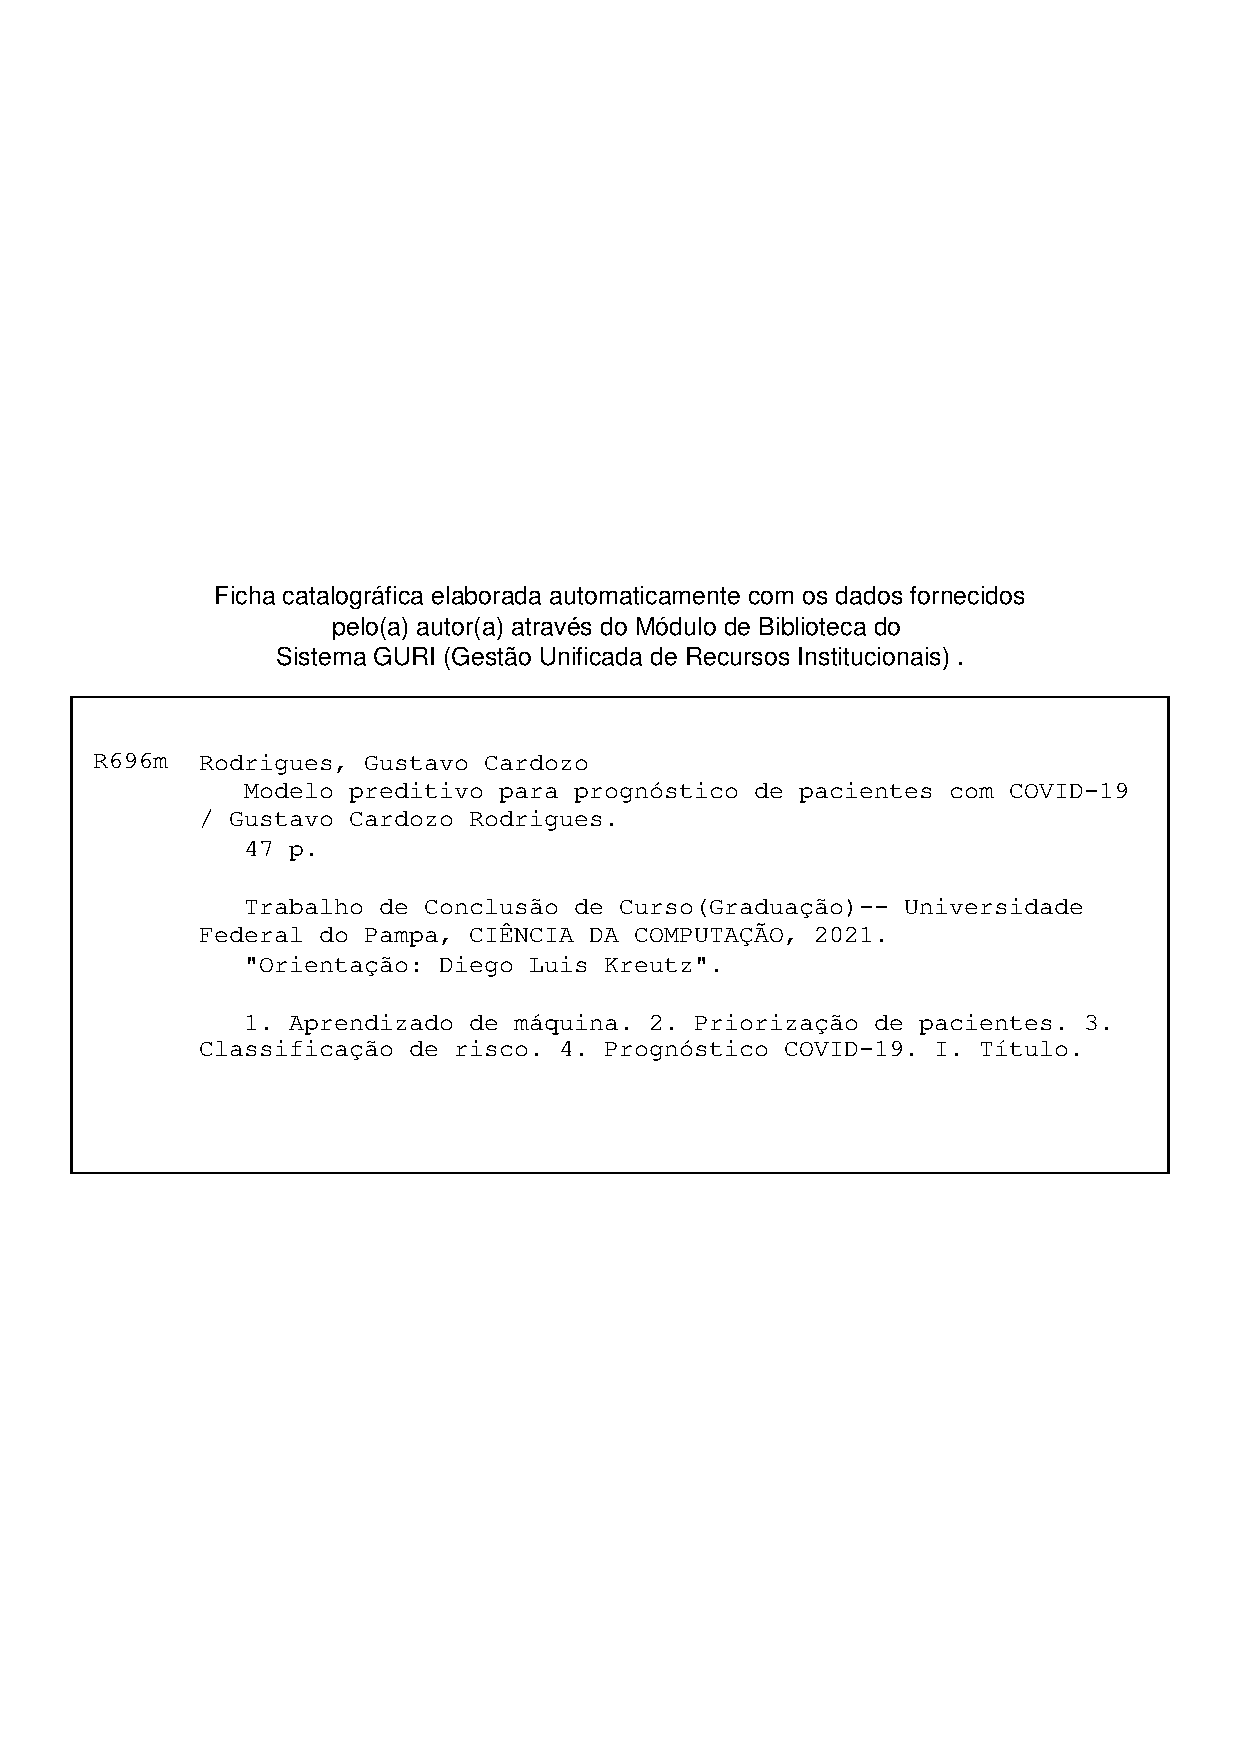
\includepdf{pretextuais/ficha_catalografica.pdf}

\begin{folhadeaprovacao}

\includepdf[page={1,2}]{pretextuais/aprovacao.pdf}


\end{folhadeaprovacao}



% -----------------------------------------------
% Dedicatória [OPCIONAL]
% -----------------------------------------------
\begin{dedicatoria}
   \vspace*{\fill}
   \begin{flushright}
     Dedico este trabalho a Deus, por ser essencial em minha vida, meu socorro bem presente na hora da tribulação. 
     Porque dele, e por ele, e para ele são todas as coisas; glória, pois, a ele eternamente. Amém!

   \end{flushright}
   \vspace*{\fill}
\end{dedicatoria}


% -----------------------------------------------
% Agradecimentos [OPCIONAL]
% -----------------------------------------------
\begin{agradecimentos}

A Deus, pela minha vida, e por ter me sustentado até aqui. 

Aos meus pais, Claudia e Paulo, aos meus irmãos Cezar e Matheus, a minha vó Nara, e a minha namorada Gabriela pelo amor e incentivo. 

Aos amigos Edinei Silva e Fernanda Souza, pelo apoio em dias trabalhosos.

%%EU NÃO VAI AGRADECER NOMINALMENTE É? jÁ VAI REPROVADO PRA BANCA AHAHAHHAA
Aos professores, pelas correções e ensinamentos que me permitiram apresentar um melhor desempenho no meu processo de formação profissional. Em especial aos amigos e orientadores, Dr. Diego Kreutz e Dr. Mirkos Martins, que acreditaram em mim, e me ajudaram a extrair o meu potencial. Muito obrigado pela paciência e pelos ``puxões de orelha'' que me deram! O meu profundo e eterno agradecimento. 

E a todos que direta ou indiretamente fizeram parte da minha formação, o meu muito obrigado.

\end{agradecimentos}

% -----------------------------------------------
% Epígrafe [OPCIONAL]
% -----------------------------------------------
\begin{epigrafe}
  \vspace*{\fill}
	\begin{flushright}
    ``O que adquire entendimento ama a sua alma; \\
        o que cultiva a inteligência achará o bem.''\\
    (BÍBLIA, Provérbios, 19, 8).
	\end{flushright}
\end{epigrafe}


% -----------------------------------------------
% Resumo [OBRIGATÓRIO]
% -----------------------------------------------
\begin{resumo}

% Objetivo
Com a criticidade da falta de leitos de unidade de terapia intensiva durante a pandemia de COVID-19, políticas para determinar quem tem acesso aos leitos foram implantadas em estados do Brasil. Objetivando mitigar a subjetividade dessas políticas, propomos o desenvolvimento e validação interna de um preditor para classificação de risco de óbito de pacientes com COVID-19 no estado do Rio Grande do Sul.
% design do estudo
Utilizamos o guia TRIPOD para explanar o desenvolvimento do modelo de aprendizagem de máquina baseado em floresta aleatória.
% participantes e tamanho da amostra
O conjunto de dados possui 604.389 registros e engloba os pacientes atendidos no Rio Grande do Sul que foram reportados através do Painel Coronavírus RS, no perído de 01 de janeiro à 08 de junho de 2021.
% variáveis preditoras e variável resposta
A variável de desfecho (\textit{outcome}) é a evolução, que informa se o paciente foi recuperado ou veio a falecer por COVID-19. No total, quatorze características foram elencadas como preditoras, sendo elas demográficas (sexo e faixa etária) e clínicas (sintomas e comorbidades). 
% análises estatísticas, resultados
O conjunto de dados de derivação possui 408.959 registros, sendo 3,18\% (n=13.005) óbitos, e o conjunto de validação possui 175.269 registros, sendo 5.574 óbitos. No conjunto de testes, o modelo classificou a chance de óbito com uma pontuação AUC-ROC de 0,981 (intervalo de confiança  de 95\% 0,981 a 0,982) e AUC-ROC de 0,970 no conjunto de validação.
% conclusões
O classificador permite estratificar com boa precisão o risco de óbito de pacientes com COVID-19 e pode contribuir na dimuinição da subjetividade na tomada de decisão no ambiente hospitalar. Entretanto, salientamos que esta é apenas uma ferramenta adicional, e todos os aspectos éticos e legais devem ser considerados na tomada de decisão médica.
\vspace{\onelineskip}

    
 \noindent
 \textbf{Palavras-chave}: Aprendizado de Máquina. Priorização de Pacientes. Classificação de Risco. Prognóstico COVID-19.
\end{resumo}


% -----------------------------------------------
% Abstract (resumo em inglês) [OBRIGATÓRIO]
% -----------------------------------------------
\begin{resumo}[Abstract]


% Objetivo
With the criticality of the lack of beds in the intensive care unit during the COVID-19 pandemic, policies to determine who has access to beds were implemented in Brazilian states. Aiming to mitigate the subjectivity of these policies, we propose the development and internal validation of a predictor for death risk classification of patients with COVID-19 in Rio Grande do Sul.
% design do estudo
We use the TRIPOD guideline to explain the development of the random forest-based machine learning model.
% participantes e tamanho da amostra
The dataset has 604,389 records and includes patients treated in Rio Grande do Sul who were reported through the Painel Coronavírus RS, in the period from January 1 to June 8, 2021.
% variáveis preditoras e variável resposta
The outcome variable is evolution, which informs whether the patient was recovered or died from COVID-19. In total, fourteen characteristics were listed as predictors, which were demographic (gender and age group) and clinical (symptoms and comorbidities). 
% análises estatísticas, resultados
The derivation dataset has 408,959 records, being 3.18\% (n=13,005) deaths, and the validation set has 175,269 records, being 5,574 deaths. In the test set, the model rated the chance of death with an AUC-ROC score of 0.981 (95\% confidence interval 0.981 to 0.982) and AUC-ROC of 0.970 in the validation set.
% conclusões
The classifier makes it possible to stratify with good precision the risk of death of patients with COVID-19 and can contribute to the reduction of subjectivity in decision-making in the hospital environment. However, we point out that this is just an additional tool, and all ethical and legal aspects must be considered in decision-making.
 \vspace{\onelineskip}
 
 \noindent
 \textbf{Key-words}: Machine Learning. Patient Priorization. Risk Stratification. COVID-19 Prognosis.
\end{resumo}


% Resumo estendido [OPCIONAL]
% \input{pretextuais/resumoest}

% -----------------------------------------------
% Listas
% -----------------------------------------------
% Figuras/Ilustrações [OPCIONAL]
%\pdfbookmark[0]{\listfigurename}{lof}
%\listoffigures*
%\cleardoublepage
% -----------------------------------------------
% Tabelas [OPCIONAL]
%\pdfbookmark[0]{\listtablename}{lot}
%\listoftables*
%\cleardoublepage
% -----------------------------------------------
% Abreviaturas [OPCIONAL] (veja o pacote acro e os exemplo acima)
%\newcommand{\lobname}{Lista de abreviaturas}
%\pdfbookmark[0]{\lobname}{lob}
%\printacronyms[include-classes=abreviaturas,name=\lobname,heading=chapter*]
%\cleardoublepage
% -----------------------------------------------
% Siglas [OPCIONAL] (veja o pacote acro e os exemplo acima)
%\newcommand{\loaname}{Lista de siglas}
%\pdfbookmark[0]{\loaname}{loa}
%\printacronyms[include-classes=acronimos,name=\loaname,heading=chapter*]
%\cleardoublepage
% -----------------------------------------------
% Símbolos [OPCIONAL] (veja o pacote nomencl e os exemplo acima)
%\renewcommand{\nomname}{Lista de símbolos}
%\pdfbookmark[0]{\nomname}{los}
%\printnomenclature
%\cleardoublepage


% -----------------------------------------------
% Sumário
% -----------------------------------------------
\pdfbookmark[0]{\contentsname}{toc}
\tableofcontents*
\cleardoublepage
% -----------------------------------------------

\begin{comment}
  %cutter={M1234x}, % INFORMAÇÃO QUE VAI NA FICHA CATALOGRÁFICA
  %cdu={100.0*01.10},  % Define o identificador CDU do documento, fornecido pela Secretaria do Curso (verificar se é necessário).
  keywords={Modelo de texto, UNIPAMPA, Latex}, % Define as palavras-chave que deverão constar na Ficha Catalográfica, separadas por vírgulas.
  firstcommitteemember={Nome membro da banca 1\\ UNIPAMPA},
  secondcommitteemember={Nome membro da banca 2\\ Instituição},
\end{comment}



% +++++++++++++++++++++++++++++++++++++++++++++++++++++++++++++++++++++++++++++++++++++++++++++++++
% ELEMENTOS TEXTUAIS
% +++++++++++++++++++++++++++++++++++++++++++++++++++++++++++++++++++++++++++++++++++++++++++++++++
% É possível usar \textual ou \mainmatter, que é a macro padrão do memoir.
\textual

% Você pode dividir o seu texto em vários arquivos. Por exemplo, um para cada seção principal do
% trabalho: introducao.tex, relacionados.tex, metodologia.tex, experimentos.tex, conclusao.tex.
%==============================================================================
\chapter{Introdução}\label{sec_introducao}
%==============================================================================


% cenário
\red{Durante a pandemia de \textit{coronavirus disease 2019} (COVID-19) os sistemas de saúde do mundo inteiro enfrentam problemas quanto a disponibilidade e alocação de recursos como respiradores e leitos de UTI (Unidade de Terapia Intensiva) \cite{latif2020leveraging} \cite{ranney2020critical}. Políticas e decisões críticas estão sendo tomadas quanto a priorização de pacientes com a doença e, em países como o Brasil, existem regras que definem quem tem direito a leitos de UTI. Em alguns lugares, devido a urgência e falta de dados mais precisos, a política tem sido priorizar as pessoas mais jovens para a ocupação dos leitos de UTI\footnote[1]{https://www.nsctotal.com.br/colunistas/dagmara-spautz/estado-oficializa-criterio-que-da-prioridade-a-mais-jovens-e-saudaveis}. Em estados como o Rio Grande do Sul, não há leitos para todos os pacientes em estado grave\footnote[2]{https://www.estado.rs.gov.br/mesmo-com-expansao-de-leitos-45-rodada-confirma-pressao-sobre-capacidade-hospitalar-e-rs-em-bandeira-preta}, consequentemente, é preciso colocar em prática políticas de priorização da alocação dos leitos com base no estado clínico do paciente.}

\red{Estudos mostram que modelos de aprendizagem de máquina (\textit{machine learning}) conseguem predizer a chance de óbito de um paciente positivo para COVID-19 com até 0,99 de pontuação AUC-ROC (\textit{Area Under the Curve - Receiver Operating Charachteristic Curve})  \cite{wynants2020prediction}.
% problema (Desafio de modelos): modelos, características e métricas
Por se tratar de um contexto crítico (pandemia e risco de vida), os modelos preditivos devem ser robustos, seguros e transparentes, sem comprometer a ética.  Um dos principais desafios é desenvolver e garantir a credibilidade destes modelos.}

% modelos
%\red{No contexto de análise preditiva, o estado da arte aponta que o algoritmo Floresta Aleatória (\textit{Random Forest}) é o mais frequentemente utilizado (Seção \ref{sec_classificacao_de_risco}). Isto ocorre devido ao fato deste método ser considerado acurado e robusto pois que conta com um alto número de árvores de decisão \cite{james2013statistical}) no processo, por não sofrer com sobreajuste e pelo seu auxílio na classificação da importância das características \cite{breiman2001random}.}

% características
%\red{Com relação as características utilizadas para ``alimentar'' o modelo, foi possível constatar que as mais utilizadas para treinamento são dados clínicos (\textit{e.g.}, sintomas e comorbidades), dados demográficos (\textit{e.g.}, idade, sexo e país de origem) \cite{iwendi2020covid, pourhomayoun2020predicting, yadaw2020clinical, chowdhury2020early, dun2020machine}, dados laboratoriais (\textit{e.g.}, amostras de sangue) \cite{cheng2020using, gao2020machine, chowdhury2020early, casiraghi2020explainable} e características radiológicas (\textit{e.g.}, imagens de radiografia) \cite{casiraghi2020explainable}. 
%Tanto os tipos de dados quanto a quantidade de características utilizadas nos estudos variam significativamente, indo de 3 \cite{yadaw2020clinical} a 99 \cite{cheng2020using} características. Por fim, ROC-AUC foi a métrica de avaliação mais utilizada nos estudos (ver detalhes na Seção \ref{sec_classificacao_de_risco})}

% problemática com população
\blue{Muitos estudos e propostas de soluções para classificação de risco refletem dificuldades nas suas aplicações ou até mesmo em como podem auxiliar no contexto médico \cite{wynants2020prediction}. Diversos modelos contém alto risco de enviesamento (\textit{i.e.}, modelo não generalista) devido ao desenvolvimento baseado em amostras pequenas da população (\textit{e.g.}, dados de apenas um hospital), métricas de avaliação inadequadas (\textit{e.g.}, acurácia para dados desbalanceados), ou pobreza de detalhes sobre o desenvolvimento e objetivo do modelo (\textit{e.g.}, omissão dos métodos utilizados) \cite{wynants2020prediction}. Devido a alta variabilidade climática, cultural e racial entre diferentes países e populações \cite{assaf2020utilization, cheng2020using, zhao2020prediction, casiraghi2020explainable} é necessário o desenvolvimento de uma solução que utilize dados de populações pouco exploradas, como é o caso do Brasil, além de utilizar métricas para avaliação do desempenho de modelos com dados desbalanceados. Por fim, para mitigar a falta de detalhes na explanação do estudo, deve-se utilizar guias que auxiliem a relatar de maneira transparente o desenvolvimento do modelo como o STARD (\textit{Standards for Reporting of Diagnostic Accuracy}) \cite{bossuyt2003stard} e o TRIPOD (\textit{Transparent Reporting of a multivariable prediction model for Individual Prognosis Or Diagnosis}) \cite{collins2015tripod}. } 

%métricas em dados desbalanceados
%\red{A acurácia é a métrica mais comumente utilizada em problemas de %classificação, embora nem sempre seja adequada, sendo potencialmente perigosa %quando usada em conjunto de dados desbalanceados \cite{guo2008class}. Se 95\% %dos dados pertencerem à majoritária (negativa/recuperação), é fácil ver que um %classificador ingênuo terá acurácia de 95\%, simplesmente prevendo a classe %negativa sempre, o que não é aceitável na prática, pois não estaremos %identificando os exemplos pertencentes à classe minoritária (positiva/óbito). 
%\red{No contexto do presente trabalho, a proporção de casos recuperados por casos de óbito no estado do Rio Grande do Sul é de aproximadamente 40:1\footnote[3]{https://covid.saude.gov.br/} (quarenta para um), para tal, precisamos utilizar métricas alternativas como a ROC-AUC, que foi a métrica mais utilizada em estudos recentes (ver detalhes na Seção \ref{sec_classificacao_de_risco}). Contudo, há métricas de avaliação de modelos de classificação binária mais informativas e com menos propensão a invesamento à classe majoritária, como é o caso da visualização da Precisão-revocação \cite{saito2015precision}.}

% objetivo do trabalho
\blue{Neste trabalho, propomos um modelo preditivo baseado em florestas aleatórias \cite{breiman2001random} para classificação de risco de óbito para pacientes confirmados de COVID-19 no estado do Rio Grande do Sul/Brasil. Utilizamos a pontuação AUC-ROC para avaliar a performance do modelo. Este é um indicador importante pois nos fornece uma medida da precisão total do modelo independente de um limiar particular \cite{fawcett2006roc}. O desenvolvimento do modelo é explanado utilizando o guia TRIPOD para atenuar o risco da falta de detalhes. Utilizamos também da validação cruzada 5-\textit{fold} para validar internamente o modelo e, desta forma, reduzir o risco de enviesamento.} %temos um modelo preditivo com menor risco de enviesamento e mais robusto (\textit{i.e} mais acurado), aliado à aplicação dos testes sobre uma população ainda pouco explorada pelos estudos (Rio Grande do Sul).

% metodologia
%\red{Para atingir o objetivo, o trabalho foi dividido em quatro etapas. A primeira etapa consiste na aquisição e análise dos dados. Na segunda etapa é realizada a limpeza e mineração de dados para a eliminação das inconsistências e dados faltantes. Na terceira etapa, o pré-processamento dos dados que antecederam a quarta etapa, que consistiu na implementação e validação do modelo preditivo.}

\red{O restante deste trabalho está organizado como segue. 
Na Seção \ref{sec_classificacao_de_risco} é apresentado o estado da arte do aprendizado de máquina aplicado ao combate da pandemia. Na Seção  \ref{sec_metodologia} é discutido o projeto do estudo, a aquisição dos dados e a construção do modelo de prognóstico. Na Seção \ref{sec_resultados} avaliamos a performance do modelo construído, bem como a sua interpretabilidade. Por fim, na Seção \ref{sec_discussao} há a discussão geral sobre as contribuições e limites do presente estudo.} % [OBRIGATORIO]
%\part{Revisão de Literatura} % Pode-se usar partes para organizar os capítulos
%%%%%%%%%%%%%%%%%%%%%%%%%%%%%%%%%%%%%%%%%%%%%%%%% 
\chapter{Estado da arte} \label{sec_classificacao_de_risco}
%%%%%%%%%%%%%%%%%%%%%%%%%%%%%%%%%%%%%%%%%%%%%%%%% 

\blue{Nesta seção é apresentado o estado da arte do aprendizado de máquina aplicado ao combate da pandemia. Aprendizagem de Máquina é um ramo da Inteligência Artificial onde sistemas computacionais podem aprender a partir de dados e identificar padrões com o mínimo de intervenção humana \cite{mitchell1997machine}. A Tabela \ref{tab_trabalhos_relacionados} apresenta o resumo de métodos de aprendizagem de máquina, métricas de avaliação e características aplicadas ao contexto da pandemia de COVID-19.
Os métodos identificados tem por objetivo auxiliar na tomada de decisão médica, incluindo prever a severidade dos casos confirmados (classificação de risco), chance de óbito ou recuperação, e chance de internação em UTI.}

\blue{Segundo os dados coletados, o método Floresta Aleatória é o mais frequentemente utilizado (aparece em 80\% dos casos).  Isto ocorre devivo ao fato deste método ser considerado acurado e robusto pois conta com um alto número de árvores de decisão no processo de treinamento, por não sofrer com sobreajuste e pelo seu auxílio na classificação da importância das características \cite{breiman2001random}. Devido às características mencionadas, utilizamos este algoritmo no processo de desenvolvimento do modelo preditivo para classificação de risco de mortalidade de pacientes com COVID-19.}

\begin{table}[!htb]  \footnotesize
\centering
\caption{Métodos de aprendizagem de máquina, métricas de avaliação e características}
\label{tab_trabalhos_relacionados}
\begin{tabular}{| p{4.0cm} | p{4.3cm} | p{2.5cm} | p{3.7cm} | }
\hline\hline
&
  \textbf{Métodos de aprendizagem de máquina usados} &
  \textbf{Características} &
  \textbf{Métricas de avaliação} \\ \hline

  
\textbf{\cite{iwendi2020covid}} & Floresta Aleatória* Intensificada (AdaBoost); Árvore de decisão; Máquina de Vetores de Suporte (SVM); Naive Bayes Gaussiano & Demográficas; Clínicas & 
Acurácia; Precisão; Revocação; F1 Score; Matriz de confusão \\ \hline
  
\textbf{\cite{pourhomayoun2020predicting}} &
  Redes Neurais Artificiais; Árvore de decisão; Floresta Aleatória*; K-vizinhos mais próximos (KNN); Regressão Logística; Máquina de Vetores de Suporte (SVM) &re
  Demográficas; Clínicas &
Acurácia; ROC-AUC;  Matriz de confusão \\ \hline
  
\textbf{\cite{zhao2020prediction}} &
  Regressão Logística &
  Clínicas &
  ROC-AUC \\ \hline
  
\textbf{\cite{yadaw2020clinical}} &
  eXtreme Gradient Boosting (XGBoost); Regressão Logística; Floresta Aleatória*; Máquina de Vetores de Suporte (SVM) &
  Demográficas; Clínicas &
  ROC-AUC \\ \hline
  
\textbf{\cite{cheng2020using}} &
  Floresta Aleatória* &
  Clínicas; Laboratoriais &
  Revocação; Especificidade; Acurácia; ROC-AUC; Matriz de confusão\\ \hline
  
\textbf{\cite{assaf2020utilization}} &
  Redes Neurais Artificiais; Floresta Aleatória*; Árvore de Decisão &
  Clínicas &
  Revocação; Especificidade; Acurácia; F1 Score; ROC-AUC;  Matriz de confusão\\ \hline
  
\textbf{\cite{gao2020machine}} &
  Regressão Logística; Máquina de Vetores de Suporte (SVM); eXtreme Gradient Boosting (XGBoost); Redes Neurais Artificiais; K-vizinhos mais próximos (KNN) &
  Clínicas; Laboratoriais &
  Razão de probabiliadde positiva; Razão de probabilidade negativa; F1 score; ROC-AUC; Matriz de confusão\\ \hline
  
\textbf{\cite{chowdhury2020early}} &
  eXtreme Gradient Boosting (XGBoost);  Regressão Logística &
  Demográficas; Clínicas; Laboratoriais &
  Revocação; Especificidade; Razão de probabiliadde positiva; Razão de probabilidade negativa; ROC-AUC; Matriz de confusão \\ \hline
  
\textbf{\cite{casiraghi2020explainable}} &
  Floresta Aleatória* &
  Radiológicas; Clínicas; Laboratoriais &
  Revocação; Especificidade; Acurácia; F1 score; ROC-AUC; Matriz de confusão \\ \hline
  
\textbf{\cite{dun2020machine}} &
  Floresta Aleatória* &
  Demográficas; Clínicas &
  -- \\ \hline
\end{tabular}
\end{table}

As principais características utilizadas para treinamento são dados demográficos (\textit{e.g.}, idade, sexo e país de origem), presentes em 50\% dos trabalhos; dados clínicos (\textit{e.g.}, sintomas e comorbidades), presentes em 100\% dos trabalhos; dados laboratoriais (\textit{e.g.}, amostras de sangue), presentes em 40\% trabalhos, onde foi possível identificar a mínima saturação de O2 como característica chave. 
Por fim, características radiológicas (\textit{e.g.}, imagens de radiografia) também aparecem como características de treinamento \cite{casiraghi2020explainable}.

Nos modelos propostos e treinados, a quantidade de características usadas varia de 3 \cite{yadaw2020clinical} a 99 \cite{cheng2020using}. 
Entretanto, foi possível observar que a idade e o sexo foram unânimes nos estudos que utilizaram de dados demográficos. 
Além disso, é importante ressaltar que nos modelos que utilizam dados clínicos, em termos de sintomas e comorbidades, todos utilizaram características relacionadas a resfriados, como febre, tosse e dispnéia.

Para entender quão bom um modelo preditivo é, existem métricas para avaliar o desempenho (ou generalização) de um método de aprendizagem de máquina \cite{amidi2020ml}. 
As métricas mais encontradas nos trabalhos foram métricas obtidas através da matriz de confusão, sendo a AUC-ROC a mais utilizada (presente em 80\% dos trabalhos), seguida por acurácia, precisão, sensibilidade, especificidade e F1 \textit{score} (presentes em 70\% dos trabalhos).

Os estudos mostram que modelos de aprendizagem de máquina conseguem prever chances de recuperação ou óbito com até 94\% de acurácia, com um F1 \textit{score} de 0.84 \cite{iwendi2020covid}. 
Essa métrica (F1 \textit{score}) auxilia na verificação do quão bom e generalista o modelo é, visto que é uma média harmônica entre a precisão (verdadeiros que realmente eram verdadeiros) e a sensibilidade (proporção dos verdadeiros positivos entre todas as observações que realmente são positivas). 
Isto demonstra a importância de outras métricas para avaliação dos modelos, além da acurácia, que é tipicamente a métrica mais utilizada em problemas de classificação binária.

Os trabalhos relacionados na Tabela \ref{tab_trabalhos_relacionados} possuem uma limitação em comum: o grupo de pacientes utilizados para treino. Um modelo de previsão aplicado em um novo sistema de saúde,
configuração ou país geralmente produz previsões que estão mal calibradas e podem precisar ser atualizadas antes que possam ser aplicadas com segurança nessa nova configuração. 
Os mesmos métodos, com outras populações ou de outros sistemas de saúde, podem levar a resultados diferentes  \cite{assaf2020utilization, cheng2020using, zhao2020prediction, casiraghi2020explainable}. 

Dados de vários países e sistemas de saúde podem permitir uma melhor compreensão da generalização e implementação de modelos de previsão em diferentes configurações e populações \cite{wynants2020prediction}. É com esta premissa que
neste trabalho serão utilizados dados abertos, as mesmas técnicas de aprendizagem de máquina, avaliação e validação do estado da arte, porém aplicadas à população do Rio Grande do Sul.




%\input{textuais/trabalhos_relacionados.tex}

%%%%%%%%%%%%%%%%%%%%%%%%%%%%%%%%%%%%%%%%%%%%%%%%%% 
\chapter{Estudo de Caso} \label{sec_estudo_de_caso}
%%%%%%%%%%%%%%%%%%%%%%%%%%%%%%%%%%%%%%%%%%%%%%%%% 

Como caso de estudo o município de Santa Maria, os dados utilizados para classificações e análise sobre COVID-19 são provenientes das plataformas governamentais e-SUS Notifica e SIVEP Gripe. 
Essas plataformas são preenchidas manualmente por profissionais da saúde durante o exercício de suas atividades diárias. 
Devido a esse fato, essas bases possuem inúmeras inconsistências e, em grande parte dos casos, não seguem as instruções publicadas pelo Ministério da Saúde \cite{instrutivoesus,instrutivosivep}. 
Como consequência, as análises manuais desses dados tornam-se inviáveis, pois tendem a erros e possuem um custo operacional alto uma vez que os profissionais da área da saúde e epidemiologia não podem gastar o seu tempo na verificação da confiabilidade dos dados, validando cada registro individualmente.
    
%%%%%%%%%%%%%%%%%%%%%%%%%%%%%%%%%%%%%%%%%%%%%%%%% 
\section{Fontes de dados}
   
%%%%%%%%%%%%%%%%%%%%%%%%%%%%%%%%%%%%%%%%%%%%%%%%% 
% esus notifica
\subsection*{eSUS Notifica}

Esta plataforma foi concebida pelo Ministério da Saúde (MS), por meio do Departamento de Informática do Sistema Único de Saúde (DataSUS), em 27 de março de 2020. O sistema, que foi desenvolvido para registro de casos de Síndrome Gripal (SG) suspeitos de COVID-19, objetiva auxiliar o trabalho de profissionais da saúde no controle e triagem dos casos, prometendo formulários simples, intuitivos e de fácil utilização. As unidades públicas e privadas devem reportar casos de síndrome gripal nesta plataforma. 
A base tabular contém 53 colunas, incluindo dados sobre sintomas, comorbidades e dados demográficos.

%%%%%%%%%%%%%%%%%%%%%%%%%%%%%%%%%%%%%%%%%%%%%%%%% 
\subsection*{SIVEP-Gripe} 
O Ministério da Saúde (MS), por meio da Secretaria de Vigilância em Saúde (SVS), realiza a vigilância da Síndrome Respiratória Aguda Grave (SRAG) no Brasil, desde a pandemia de Influenza A (H1N1) em 2009. 
% Esta vigilância foi implantada na rede de influenza e outros vírus respiratórios. 
Recentemente, em 2020, o monitoramento da infecção humana causada pelo novo Coronavírus foi incorporada na rede de vigilância da influenza e outros vírus respiratórios. 
O Sistema de Informação da Vigilância Epidemiológica da Gripe (SIVEP-Gripe) contém registros de pacientes hospitalizados sob suspeita (ou diagnóstico) que caracterizam quadros de alguma síndrome respiratória aguda grave. 
Unidades de Vigilância Sentinela de Síndrome Gripal devem reportar casos seguindo fluxos estabelecidos pelo Ministério da Saúde.
As unidades sentinelas de influenza são aquelas unidades ou serviços de saúde já implantados e cadastrados no Cadastro Nacional de Estabelecimentos de Saúde (CNES) e no SIVEP-Gripe, que atuam na identificação, notificação, investigação e diagnóstico de casos suspeitos e confirmados. 
Todos os hospitais públicos ou privados devem reportar casos de SRAG que estão hospitalizados. 
A base de dados é estruturada e contém 73 colunas, incluindo dados sobre sintomas, comorbidades e dados demográficos (anonimizados). 
Essa base possui valores categóricos como ``números mágicos'', onde um número corresponde a uma característica descrita em um dicionário de dados.

Antes de começar o processo de limpeza descrito no presente trabalho, é necessário fazer uma união dos dados e-SUS Notifica e SIVEP-Gripe. 
%Esta união é um ponto importante para o trabalho de limpeza, normalização e processamento dos dados para contagem de casos e identificação de inconsistências. 
Como casos confirmados no e-SUS Notifica podem evoluir e agravar-se, resultando em hospitalizações, estes passam a ser reportados e atualizados apenas no SIVEP-Gripe. 
Além disso, há os casos de hospitalizações diretas, ou seja, que não passaram pelo e-SUS Notifica. 
Estes exemplos ilustram a necessidade de união dos dados de ambas as bases para realizar uma análise completa e detalhada dos casos suspeitos ou confirmados de COVID-19 no município.

%%%%%%%%%%%%%%%%%%%%%%%%%%%%%%%%%%%%%%%%%%%%%%%%% 
\section{Inconsistências nos dados} \label{subsec_incons_dados}

% problema na alimentação das bases
Embora vários instrutivos tenham sido publicados por meio dos canais de comunicação do MS, os frequentes atendimentos emergenciais acarretam em registros de notificação sendo parcialmente preenchidos, muitas vezes não dispondo os dados requeridos do paciente atendido (\textit{e.g.} falta da data do início dos sintomas, mesmo sintomáticos). Alguns registros de pacientes não são únicos, existe duplicidade no cadastro de atendimento no e-SUS Notifica, pois um mesmo paciente pode ser atendido por dois recepcionistas e cada um gera um registro distinto, com identificador diferente. Ou também, há registros de um mesmo paciente em datas diferentes, caracterizando mais de um episódio de suspeitas. Com o entendimento disso, é sabido que para a contagem de confirmação, exclusão ou óbito de um caso, apenas um registro deste paciente é suficiente (ver Seção \ref{subsec_limpeza}).

% Dados ausentes
As duas principais bases de dados governamentais apresentam desafios estatísticos significativos para o  município de Santa Maria. 
Por exemplo, a ausência de informações (\textit{e.g.} data da coleta da amostra e sintomas do paciente) e as inconsistências de dados (\textit{e.g.} data do início dos sintomas posterior ao resultado do teste) podem comprometer a validade dos resultados e levar a análises equivocadas. 

% motivos dos dados ausentes
A falta de dados, que podem ser expressivos na análise, pode ter diferentes causas, como a falta de coleta real (\textit{e.g.}, paciente nunca ter sido questionado sobre histórico de asma) ou por falta de coleta devido à atendimentos emergenciais (\textit{e.g.,} paciente foi questionado sobre asma, mas a resposta nunca foi registrada no prontuário). 
Alguns profissionais da saúde reclamam que uma documentação eletrônica discreta mais completa requer trabalho adicional; às vezes sem benefícios imediatos ou óbvios para o atendimento ao paciente. 
Estudos apontam que este é um dos principais motivos da falta de dados ou documentação relacionada à pacientes que não apresentam o sintoma, comorbidade ou situação \cite{wells2013strategies}. 
Ao invés de registrar um valor negativo no sistema, os profissionais da saúde simplesmente omitem a informação e registram apenas os positivos.
    
% problemas em dados textuais
As bases e-SUS Notifica e SIVEP-Gripe possuem diversos dados estruturados, muitos deles representados como valores numéricos ou discretos (\textit{i.e.}, categoria pré-definida), e também dados textuais.
Enquanto que os campos numéricos são fáceis de processar automaticamente, os campos com dados textuais (\textit{e.g.}, nota sobre outros sintomas ou condições descrito pelo médico) são difíceis de analisar quantitativamente devido as variações da expressão humana, erros gramaticais, uso de siglas, abreviações e jargões, e o potencial para diferentes interpretações da mesma frase dependendo do contexto.

% problema específico
Resumidamente, os campos textuais das duas bases possuem informações ambíguas em relação a campos estruturados referentes a condições, comorbidades e sintomas (ver Seção \ref{subsec_limpeza}). 
Por exemplo, há um campo onde os profissionais da saúde podem descrever sintomas diferentes dos destacados nos sistemas. 
Porém, em alguns casos, como febre e tosse, os campos específicos dos sintomas estão sendo ignorados e o registro está sendo realizado no campo descritivo geral.

% correção
Abordar adequadamente o problema dos dados ausentes nos registros eletrônicos de saúde é uma tarefa complicada pelo fato de ser frequentemente difícil diferenciar entre dados ausentes e um valor realmente negativo. 
Um exemplo é um caso documentado como não apresentando dispneia. 
É difícil saber se o paciente não apresentou o sintoma ou se o prestador de serviço hospitalar simplesmente não documentou o episódio. 
Para mitigar a perda de dados nesse tipo de sistemas, existem diferentes abordagens, como o aumento da documentação de dados estruturados, a redução de erros de entrada de dados através de interfaces mais elaboradas e a utilização de análise automatizada de texto \cite{wells2013strategies} (adotada no presente trabalho). 

\begin{figure}[ht]
\caption{Quadro de Síndrome Gripal}
\centering % para centralizarmos a figura
\includegraphics[width=12cm]{figuras/quadro_sg.png}
\label{figura_sg}
\end{figure}
    
\begin{figure}[ht]
\caption{Quadro de Síndrome Respiratória Aguda Grave}
\centering % para centralizarmos a figura
\includegraphics[width=12cm]{figuras/quadro_srag.png}
\label{figura_srag}
\end{figure}
    
As Figuras \ref{figura_sg} e \ref{figura_srag} representam os algoritmos definidos pelo Ministério da Saúde que caracterizam um caso como SG ou SRAG \cite{definicaoMinisterioSaudeSG}.
O entendimento destes algoritmos é necessário para a compreensão das características que devem ser analisadas a fim de encontrar incoerências com a definição do próprio MS. 
Um aspecto a observar é que não existem campos correspondentes aos sintomas batimentos de asa de nariz, cianose, tiragem intercostal, desidratação, inapetência, dor de cabeça, distúrbio olfativo, distúrbio gustativo, obstrução nasal, síncope, confusão mental, sonolência, diarreia, dispneia/desconforto respiratório, pressão torácica e dessaturação, que são necessários para a categorização do caso como SG ou SRAG. 
Isto significa que é necessário minerar os textos de descrição de sintomas para extrair essas informações de sintomas específicos.
    
\begin{figure}[ht]
    \caption{Fluxo esperado e obtido de evolução de casos}
    \centering % para centralizarmos a figura
    \includegraphics[width=12cm]{figuras/fluxo_de_evolucaocaso.png}
    \label{figura_evolucao_caso}
\end{figure} % 

A Figura \ref{figura_evolucao_caso} resume o comportamento esperado de evolução dos casos. 
Como pode ser observado, o fluxo representa o senso comum sobre a evolução de doenças como a causada pelo vírus Sars-CoV-2 (vírus causador da COVID-19). 
Entretanto, durante a pandemia e devido a fatores já mencionados, foram constatadas discrepâncias significativas nas bases governamentais (como pode ser observado nas setas pontilhadas em laranja na figura), o que pode levar a resultados equivocados sobre a evolução dos casos de COVID-19. Algumas das discrepâncias encontradas nos dados das bases governamentais, são detalhadas a seguir.

\begin{itemize}

       \item Foram encontrados casos que evoluíram para `Ignorado', porém, no registro de resultado do teste apontava para `Positivo';
        \item Foram encontrados casos que evoluíram para `Cura' ou `Óbito', mas sem resultado do teste ou com resultado do teste apontando para `Negativo';
        \item Foram encontrados casos de pessoas que evoluíram para `Em Tratamento Domiciliar', porém, com resultado do teste apontando para `Negativo';
        \item Inconsistências observadas em casos descartados, considerando que alguns deles evoluíram para `Óbito', `Cura' ou `Em Tratamento Domiciliar', comportamento este considerado anormal, visto que todos possuem resultado do teste apontando para `Negativo'. Isto ocorre também devido ao fato de o resultado do teste `Negativo' no SIVEP-Gripe poder significar negatividade para Influenza, mas não para COVID-19.
        
\end{itemize}

%%%%%%%%%%%%%%%%%%%%%%%%%%%%%%%%%%%%%%%%%%%%%%%%% 
\section{Desafios}
 
%%%%%%%%%%%%%%%%%%%%%%%%%%%%%%%%%%%%%%%%%%%%%%%%% 
 % DESAFIO DE CONTEXTO
\subsubsection*{De contexto}

Um dos obstáculos iniciais do projeto foi compreender o contexto. 
Por se tratarem de dados relacionados à saúde, a compreensão sobre jargões ou nomes técnicos sobre sintomas, comorbidades ou doenças tem um impacto significativo na manipulação dos dados. 
Um exemplo prático é o nome da popularmente conhecida ``dor-de-cabeça'', que em contexto médico, é denominada cefaleia. 
Um segundo exemplo são os termos sobre distúrbios que não eram previamente conhecidos pelos autores, como ageusia e anosmia -- distúrbios gustativos e olfativos, respectivamente. 
Além disso, há diversos outros nomes técnicos sobre tipos de testes, como os de critério laboratorial: Ensaio imunoenzimático (ELISA), Imunocromatografia (teste rápido),  e Imunoensaio por Eletroquimioluminescência (ECLIA). 
Como um último exemplo, existem termos de contexto que não são comuns aos profissionais alheios à área da saúde, como ``Detectável'' ou ``Reagente'', que significam resultado positivo para algum agente etiológico (\textit{i.e.} positivo para alguma SG ou SRAG). 
\textit{Detectável} diz respeito aos testes por biologia molecular, onde o entendimento sobre os tipos de sorologias precisam ser estudados e compreendidos.
Por outro lado, \textit{reagente} remete a testes imunológicos e testes de pesquisa de antígeno (rápidos). Para o entendimento desses testes, conhecimentos sobre as imunoglobulinas (IgM, IgG e IgA) -- que são anticorpos que aparecem após um tempo do agente etiológico no corpo do paciente -- tiveram que ser estudados. 

 
 %%%%%%%%%%%%%%%%%%%%%%%%%%%%%%%%%%%%%%%%%%%%%%%%% 
% DESAFIO DE COMUNICAÇÃO
\subsubsection*{De comunicação}

Como a equipe de epidemiologia estava sob pressão contínua devido à pandemia em curso, houve uma dificuldade de manutenção de diálogos frequentes, o que levou a atrasos e contratempos relacionados a compreensão dos detalhes específicos do contexto. 
Frequentemente, a tarefa de comunicar as mudanças feitas na plataforma para os interessados em sua utilização era bastante desafiadora, considerando a inevitabilidade da utilização de termos técnicos específicos da computação e o debate acerca das reais necessidades da equipe epidemiológica de Santa Maria. Já que esse é um problema crítico, decisões rápidas sobre soluções tiveram de serem tomadas, e por isso vários problemas só foram compreendidos em um estágio relativamente avançado do trabalho, sendo necessário, por vezes, uma reunião com todas as partes interessadas com o objetivo de redefinir o escopo.
 
%%%%%%%%%%%%%%%%%%%%%%%%%%%%%%%%%%%%%%%%%%%%%%%%% 
 % desafio tecnico de mudança nas bases
\subsubsection*{Técnicos}

Por se tratarem de sistemas em homologação, como é o caso do e-SUS Notifica, ou adaptados a um novo contexto, como é o caso do SIVEP-Gripe, essas plataformas estiveram em constante evolução no panorama criado pela pandemia. 
Como a plataforma SIVEP-Gripe foi desenvolvida para registrar casos de alguma SRAG, possuir o dado de ``positivo'' para resultado do teste não caracteriza confirmação para COVID-19, mas sim que houve a confirmação para algum agente etiológico (\textit{e.g.}, Influenza). 
Outro aspecto a ser observado é que, em algumas versões, o fato da negativação para o resultado do teste apenas informava que o paciente testou negativo para Influenza, mas ainda poderia ter resultado positivo para COVID-19. 
Como consequência, campos extras começaram a ser adicionados aos sistemas no decorrer da pandemia. 
Durante o desenvolvimento deste trabalho, três mudanças na forma de organizar os dados nos sistemas e-SUS Notifica e SIVEP-Gripe ocorreram, o que resultou em re-trabalho de limpeza de dados e extração de informações.

%\part{Resultados}
%\input{textuais/outrospontos} % Outro capítulo
%\bookmarksetup{startatroot} % Usar se o próximo capítulo não pertencer à parte anterior e não existir uma parte nova

%==============================================================================
\chapter{Metodologia}\label{sec_metodologia}
%==============================================================================

\section{Projeto do Estudo}

\blue{Objetivando mitigar problemas relacionados ao risco de enviesamento por pobreza no relatório sobre o desenvolvimento do modelo \cite{wynants2020prediction}, a metodologia para o desenvolvimento e exposição dos resultados seguem o guia TRIPOD \cite{collins2015tripod}. Este é um \textit{checklist} sobre pontos essenciais que um estudo de diagnóstico ou prognóstico deve relatar quando estiver explanando o desenvolvimento de um modelo preditivo multivariado. O \textit{checklist} TRIPOD deste trabalho pode ser encontrado no apêndice \ref{appendix:tripod}.}

%\section{Participantes}

%\red{O estudo engloba todos os pacientes que foram reportados estado do Rio Grande do Sul que foram reportados pelos dois sistemas de notificações oficiais do Ministério da Saúde no monitoramento da doença: o e-SUS Notifica \cite{instrutivoesus} e o Sistema de Informação da Vigilância Epidemiológica da Gripe (Sivep-Gripe) \cite{instrutivosivep}.} \red{Rio Grande do Sul é um estado localizado ao sul do Brasil, e contém uma população estimada de 11.422.973 pessoas\footnote[4]{https://cidades.ibge.gov.br/brasil/rs/panorama}.}

\section{Participantes}

\red{Para o desenvolvimento, treino e validação do modelo preditivo, utilizamos dados anonimizados provenientes do Painel Coronavírus RS\footnote[3]{https://ti.saude.rs.gov.br/covid19/}. A escolha dos dados foi devido a acessibilidade dos mesmos e também por estarem isentos das leis de proteção aos dados \cite{lgpd2019errc}.} 
\red{Neste estudo, utilizamos um conjunto de dados com 604.389 registros (observações) de casos confirmados de COVID-19. O conjunto de dados original contém um total de 30 variáveis em nível-paciente, incluindo dados demográficos (\textit{e.g.}, sexo e faixa-etária), clínicos (\textit{e.g.}, tosse e dispneia) e temporais (\textit{e.g.}, data do início dos sintomas), compreende o perído de 01 de janeiro de 2021 à 08 de junho de 2021.}

\subsection{Engenharia de características}

\blue{A Figura \ref{figura_data_selection} retrata o fluxo da seleção dos dados elegíveis para este estudo. No conjunto de dados, existem registros de pacientes que vieram a óbito por causas distindas da COVID-19 (20 [ < 0,01\%]), e também há aqueles cujo parecer evolutivo ainda não era conhecido naquele momento, ou seja, que ainda estavam em acompanhamento (17.724 [ < 3\%]).  Há também registros com informação faltante do sintoma dispneia (2.418 [< 0,5]\%). Optamos por remover os registros com informações faltantes e aqueles que não possuem informação relevante para o estudo (\textit{i.e.}, óbitos por outras causas ou em acompanhamento). Ao final da seleção, dos 604.389 registros inicais, 584.228 permaneceram na base para prosseguir o estudo. }

\blue{Além das características iniciais do conjunto de dados\footnote[4]{https://ti.saude.rs.gov.br/covid19/api}, outras seis características foram extraídas do campo textual ``CONDICOES'' (campo pré-existente no conjunto de dados), a saber: cardiopatia, diabetes, doença respiratória, problema renal, obesidade e doença cromossômica.} \blue{Como a variável ``Raça/cor'' possuía 19,98\% (n=116.752) de dados faltantes, sendo estes 58\% dos óbitos totais (n=10.889), e devido ao decréscimo da pontuação do modelo ao adicioná-la como preditora (ver Seção \ref{sec_resultados}), optamos por sua remoção do conjunto de dados.}

\purple{Utilizamos da codificação por rótulo (\textit{label encoding)} nas variáveis pois algoritmos de aprendizagem de máquina performam algebra linear no processo de treinamento \cite{chatfield2011encoding}. Como a distribuição das preditoras é binária, transformamos ``SIM'' para 1 e ``NÃO'' para 0. A única exceção no processo é da variável qualitativa ordinal ``FAIXAETARIA''. Neste caso, cada faixa-etária foi codificada com um número, a saber: ``< 1'': 0; ``01 a 04'': 1; ``05 a 09'': 2; ``10 a 14'': 3; ``15 a 19'': 4; ``20 a 29'': 5, ``30 a 39'': 6; ``40 a 49'': 7; ``50 a 59'': 8; ``60 a 69'': 9; ``70 a 79'': 10; ``80 e mais'': 11.}

\begin{figure}[H]
\caption{Fluxo de seleção dos participantes}
\centering % para centralizarmos a figura
\includegraphics[width=\textwidth]{figuras/fluxo_selecao_participantes.png}
\label{figura_data_selection}
\end{figure}

% variável resposta (dependente) 
\section{Variável resposta}

\red{O principal objetivo do trabalho é prever a chance de óbito entre pacientes positivos de COVID-19. Esta análise prognóstica é importante para a priorização dos pacientes na alocação dos recursos hospitalares. Os dados coletados possuem a informação relacionada a evolução do paciente na variável ``EVOLUCAO''. \purple{Esta variável é dicotômica -- ``ÓBITO'' (1) se o paciente faleceu, e ``RECUPERADO'' (0) caso contrário -- e nos} permite a criação de um modelo de aprendizagem de máquina para classificar os pacientes quanto à sua chance de falecimento, pois informa quais e quantos foram recuperados ou vieram a óbito por COVID-19. }

% variaveis preditoras (independente)
\section{Variáveis Preditoras}

%\blue{Os dados iniciais da base de dados são como segue: a idade dos pacientes é definida em categorias (< 1, 01 a 04, 05 a 09, 10 a 14, 15 a 19, 20 a 29, 30 a 39, 40 a 49, 50 a 59, 60 a 69, 70 a 79, 80 e mais). Raça foi classificada como branca, preta, parda, indígena e amarela. Os sintomas são febre, tosse, garganta, dispneia e a unica condição/comorbidade previamamente existente na base, é a informação sobre gestante. Todos os dados-padrão disponíveis da fonte de dados, podem ser consultados no dicionário de dados disponibilizado pelo Painel Coronavírus RS\footnote[6]{https://ti.saude.rs.gov.br/covid19/api}.}

 \red{As variáveis candidatas para preditoras foram selecionadas baseando-se em um dos critérios comuns \cite{collins2015tripod}: variáveis clínicas conhecidas de diagnóstico comum relacionado a pneumonia ou quadros gripais. Após a extração das novas características e remoção de campos que não são candidatos a variáveis preditoras (\textit{i.e.}, datas e códigos), os dados clínicos, demográficos e categóricos resultantes e que foram utilizados no estudo podem ser vistos na Tabela \ref{tab_dados_limpos}.}


\begin{table}[H]
\caption{Variáveis}
\label{tab_dados_limpos}
\begin{tabular}{lll}
\hline
Nome                  & Descrição                                                                                    & Tipo                   \\ \hline
SEXO                  & Sexo                                                                             & Binária/Demográfica    \\ \hline
FAIXAETARIA           & Faixa etária                                                                     & Categórica/Demográfica \\ \hline
EVOLUCAO              & \begin{tabular}[c]{@{}l@{}}Qual o parecer \\ evolutivo do paciente?\end{tabular}             & Binária/Alvo           \\ \hline
FEBRE                 & Sintomas de febre                                                                   & Binária/Clínica        \\ \hline
TOSSE                 & Sintomas de tosse                                                                   & Binária/Clínica        \\ \hline
GARGANTA              & \begin{tabular}[c]{@{}l@{}}Sintomas de dor de garganta\end{tabular}              & Binária/Clínica        \\ \hline
DISPNEIA              & \begin{tabular}[c]{@{}l@{}}Sintomas de dispnéia/ \\ falta de ar\end{tabular}       & Binária/Clínica        \\ \hline
GESTANTE              & O paciente é gestante?                                                                       & Binária/Clínica        \\ \hline
SRAG                 & \begin{tabular}[c]{@{}l@{}}O quadro clínico se caracteriza \\ como Sindrome Respiratória \\ Aguda Grave?\end{tabular} & Binária/Clínica \\ \hline
CARDIOPATIA           & \begin{tabular}[c]{@{}l@{}}O paciente possui alguma \\ doença cardíaca crônica?\end{tabular} & Binária/Clínica        \\ \hline
DIABETES              & O paciente possui diabetes?                                                                  & Binária/Clínica        \\ \hline
DOENCA\_RESPIRATORIA & \begin{tabular}[c]{@{}l@{}}O paciente possui alguma \\ doença respiratória crônica?\end{tabular}                      & Binária/Clínica \\ \hline
PROBLEMA\_RENAL       & \begin{tabular}[c]{@{}l@{}}O paciente possui \\ problema renal?\end{tabular}                 & Binária/Clínica        \\ \hline
OBESIDADE             & O paciente é obeso?                                                                          & Binária/Clínica        \\ \hline
DOENCA \_CROMOSSOMICA & \begin{tabular}[c]{@{}l@{}}O paciente possui \\ doença cromossômica?\end{tabular}            & Binária/Clínica        \\ \hline
\end{tabular}
\end{table}

% statistical methods
\section{Métodos Estatísticos}

\subsection{Análise descritiva}

\blue{Para entendermos sobre possíveis características que expliquem o risco de óbito, performamos análises descritivas dos preditores por cada grupo e apresentamos os resultados em quantidade e proporção de óbitos. Possíveis correlações foram analisadas utilizando o coeficiente de Pearson \cite{benesty2009pearson} e a importância relativa das características foi analisada através do grau de impureza de Gini \cite{menze2009gini} (\textit{i.e.}, a importância da característica para o modelo).}

\subsection{Análise preditiva}

\blue{Aplicamos um algoritmo de aprendizagem de máquina para prever a chance de óbito entre pacientes confirmados com COVID-19. Para a implementação, análise estatística, avaliação e validação dos modelos, utilizamos a linguagem Python 3, juntamente com as bibliotecas para aprendizagem de máquina: Scikit-learn \cite{pedregosa2011scikit} (floresta aleatória), e de manipulação e visualização de dados Pandas \cite{pandas2010}, Numpy \cite{2020NumPy-Array} e Seaborn \cite{hunter2007matplotlib}.} 

Para garantir a reproducibilidade do experimento, definimos arbritrariamente a semente 777 para embaralhar o conjunto de dados inicial. Utilizamos uma divisão pseudo-aleatória (\textit{random split}) de 70\%/30\%, a partir dos dados iniciais, sendo 70\% utilizado para treinos e testes, e os 30\% restante, para validação interna do modelo \cite{james2013statistical}. 
Avalimamos a performance/discriminação do modelo através da área sobre a curva ROC (AUC-ROC). A pontuação AUC-ROC pode assumir valores de 0 a 1, onde um valor de 0 indica um modelo que erra todas as predições e 1 reflete um teste perfeito de predição. Em geral, um valor de 0,5 sugere que o modelo não tem capacidade de discriminação (\textit{i.e.}, não consegue diferenciar pacientes que vieram a óbito dos recuperados); 0,7 a 0,8 é considerado aceitável; 0,8 a 0,9 é ótimo; e valores acima de 0,9 são considerados excelentes \cite{mandrekar2010receiver}.

Por se tratar de um conjunto de dados desbalanceado, utilizamos da técnica de subamostragem (\textit{under-sampling}, do inglês) para balancear os dados de treino, e então confrontar com o treinamento sem balanceamento para detectar melhorias \cite{anand2010approach}. Esta técnica consiste em selecionar, pseudo-aleatóriamente, pequenas fatias da classe majoritária (recuperado), a fim de igualar à quantidade de dados pertencentes a classe minoritária (óbito). Utilizamos da pesquisa de grade por validação cruzada (\textit{gridsearch cross validation}) para encontrar os melhores hiperparâmetros para o modelo - incluindo a quantidade de árvores de decisão (\texttt{n\_estimators}) e a profundidade máxima de cada árvore (\texttt{max\_depth}) \cite{krstajic2014cross} - que maximizassem a pontuação AUC-ROC nos dados de treino.

\subsection{Validação do modelo}
\blue{Para validação interna do modelo, utilizamos da técnica \textit{K-Fold Cross Validation}, que consiste em dividir o conjunto de dados em K dobras (\textit{folds}). A função de previsão é aprendida usando K-1 dobras, e a dobra deixada de fora é usada para teste. Optamos por utilizar sua variação estratificada (\textit{stratified K-Fold Cross Validation}), ou seja, na adaptação para conjuntos de dados desbalanceados, pois mantém a proporção original de cada classe na etapa de teste.
Geralmente, realiza-se a validação cruzada k-fold usando k = 5 ou k = 10, uma vez que estes valores produzem estimativas de taxa de erro de teste que não sofrem de viés ou variância excessivamente altos \cite{james2013statistical}. Por padrão, a biblioteca Scikit-learn \cite{pedregosa2011scikit} utiliza K = 5, e por isso decidimos manter este valor.}




%%%%%%%%%%%%%%%%%%%%%%%%%%%%%%%%%%%%%%%%%%%%%%%%% 
\chapter{Resultados} \label{sec_resultados}
%%%%%%,
%%%%%%%%%%%%%%%%%%%%%%%%%%%%%%%%%%%%%%%%%%% 

% caracteristicas dos pacientes diagnosticados com COVID-19
\section{Participantes}

\blue{O perfil dos participantes é apresentado na Tabela \ref{tab_dados_perfil}. Do conjunto de dados utilizado no estudo, 565.649 (96,82\%) casos possuem evolução conhecida como recuperação, e 18.579 (3,18\%) são casos que tiveram óbito comprovado por COVID-19, onde a taxa de letalidade geral é de 3,07\% (n=18.579). Dos casos confirmados, pouco mais da metade é do sexo feminino (53,10\%, n=310.263), tendo o sexo masculino a maior taxa de letalidade proporcional (3,6\%, n=9.889). Entre as faixa-etárias, a maior concentração está entre 30 e 39 anos (20,86\%), sendo a faixa superior aos 70 anos a mais letal (43.74\%, n=7.909). Dentre os sintomas, destacamos a falta de ar/dispnéia como o sintoma com a maior taxa de letalidade (17,49\%, n=15.676). Em contra-ponto, a dor-de-garganta é o sintoma apresentado que possui a menor taxa de letalidade (1,39\%, n=2.952). }

% Please add the following required packages to your document preamble:
% \usepackage{multirow}
% \usepackage{longtable}
% Note: It may be necessary to compile the document several times to get a multi-page table to line up properly
\begin{longtable}{lllll}
\caption{Dados dos participantes}
\label{tab_dados_perfil}\\ \hline
Nome do atributo                                              &               & Infectados  & Óbitos & Proporção (\%) \\ \hline
\endfirsthead
%
\endhead
%
\multirow{2}{*}{SEXO}                                          & Masculino     & 273.965 & 9889         & 3,60           \\
                                                               & Feminino      & 310.263 & 8.690         & 2,80           \\ \hline
\multirow{12}{*}{FAIXA\_ETARIA}                                 & \textless{}1  & 4.133   & 4            & 0,09           \\
                                                               & 01 a 04       & 7.403   & 4            & 0,05           \\
                                                               & 05 a 09       & 9.267   & 2            & 0,02           \\
                                                               & 10 a 14       & 13390  & 5            & 0,03           \\
                                                               & 15 a 19       & 30.292  & 19           & 0,06           \\
                                                               & 20 a 29       & 108.501 & 225           & 0,20           \\
                                                               & 30 a 39       & 121.926 & 758          & 0,62           \\
                                                               & 40 a 49       & 104.102 & 1.716          & 1,64           \\
                                                               & 50 a 59       & 88.424  & 3.138         & 3,54           \\
                                                               & 60 a 69       & 57.058  & 4.799         & 8,41           \\
                                                               & 70 a 79       & 27.233  &   4.516       & 16,58          \\
                                                               & 80 e mais     & 12.490  & 3.393         & 27,16          \\ \hline
FEBRE                                                          & Sim  & 198.357 & 8.909  & 4,49 \\
                                                               & Não           & 385.871 & 9.670         & 2,50           \\ \hline
TOSSE                                                          & Sim   & 270.337 & 10.873         & 4,02           \\
                                                               & Não           & 313.891 & 7.706         & 2,45           \\ \hline
GARGANTA                                                       & Sim  & 211.297 &  2.952  & 1,39           \\
                                                               & Não & 372.931 & 2.952        & 4,19           \\ \hline
DISPNEIA                                                       & Sim           & 89.606 & 15.676        & 17,49          \\
                                                               & Não           & 494.622 & 2.903         & 0,58           \\ \hline
GESTANTE                                                       & Sim           & 3.157   & 47           & 1,48           \\
                                                               & Não           & 581.071 & 18.532        & 3,18           \\ \hline
                                                               
SRAG                                                       & Sim           & 51.691   & 18.579           & 35,94           \\
                                                               & Não           & 532.537 & 0        & 0,0           \\ \hline
CARDIOPATIA                                                    & Sim           & 16.981  & 7.728         & 45,50          \\
                                                               & Não           & 556.396 & 10.851         & 1,91          \\ \hline
DIABETES                                                       & Sim           & 22.627  & 5.593         & 24,71          \\
                                                               & Não           & 561.601 & 17.034         & 2,31           \\ \hline
DOENCA\_RESPIRATORIA                                           & Sim           & 3.566   & 1.552         & 43,52          \\
                                                               & Não           & 563.635 & 17.027        & 2,93           \\ \hline
PROBLEMA\_RENAL                                                & Sim           & 2254   & 861         & 38,19          \\
                                                               & Não           & 581.974 & 17.718        & 3,04          \\ \hline
OBESIDADE                                                      & Sim           & 10.855   & 2.868         & 26,42          \\
                                                               & Não           & 573.373 & 15.711        & 2,74           \\ \hline
DOENCA\_CROMOSSOMICA                                           & Sim           & 141    & 83           & 41,13          \\
                                                               & Não           & 584.087 & 18.521        & 3,17           \\ \hline
\end{longtable}


\section{Desenvolvimento do modelo}
\red{Aplicamos o algoritmo de Floresta aleatória, utilizando 100 árvores de decisão (\texttt{n\_estimators}) no processo e com 4 de profundidade máxima (\texttt{max\_depth}), pois foram os melhores hiperparâmetros retornados pela busca em grade com validação cruzada (k = 5). Como o conjunto de dados de teste é desbalanceado, possuindo 395.954 (96,82\%) casos recuperados e 13.005 (3,18\%) óbitos, optamos por utilizar da técnica de subamostragem aleatória (\textit{random under sampling}) \cite{anand2010approach} nos dados de treino. }

\blue{O coeficiente de correlação de Pearson entre as variáveis independentes pode ser observado na Figura \ref{figura_corr}. Podemos constatar uma variação de -0,8 a 0,6, e que as variáveis que possuem uma maior dependência (>= 0.2) com a variável resposta (EVOLUCAO) são SRAG, DISPNEIA, CARDIOPATIA, DIABETES, DOENCA\_RESPIRATORIA e OBESIDADE (\textit{i.e.}, variáveis que possuem maior correlação). E de acordo com grau de impureza de Gini, constatamos a influência relativa das \textit{top} 5 características na classificação predita pelo modelo, a saber: SRAG, FAIXAETARIA, CARDIOPATIA, DISPNEIA e DIABETES (Figura \ref{figura_feature_importance}).}

\begin{figure}[H]
\caption{Matriz de correlação de Pearson}
\centering % para centralizarmos a figura
\includegraphics[width=\textwidth]{figuras/corr.png}
\label{figura_corr}
\end{figure}
\begin{figure}[H]
\caption{Índice de impureza de Gini}
\centering % para centralizarmos a figura
\includegraphics[width=14cm]{figuras/feature_importance.png}
\label{figura_feature_importance}
\end{figure}

\red{O fluxo geral para o uso do modelo proposto pode ser visualizado na Figura \ref{figura_geral}. Primeiramente, os dados clínicos e sintomas do paciente são coletados (A) e inseridos no modelo já treinado (B). Com o desfecho predito pelo modelo (C), o profissional da saúde em atividade (D) pode basear-se para tomar a decisão se aquele indivíduo pode ou não ocupar a vaga de leito de UTI (E).}

\begin{figure}[H]
\caption{Fluxo de uso do modelo}
\centering % para centralizarmos a figura
\includegraphics[width=\textwidth]{figuras/fluxo_geral.png}
\label{figura_geral}
\end{figure}

\section{Avaliação e Validação do modelo}

O conjunto inicial dos dados possuía 584.228 registros e um total de 18.579 óbitos. O conjunto de treino e teste possui 408.959 registros, sendo 3,18\% (n=13.005) óbitos. O conjunto de validação possui a mesma distribuição, sendo 5.574 óbitos. A Figura \ref{figura_train_test} ilustra a divisão dos dados em cada etapa de treino, teste e validação. Os valores das pontuações médias após a validação cruzada (5-V.C.) do modelo de floresta aleatória, juntamente com seus intervalos de confiança com nível de confiança de 95\% (I.C. = 95\%) podem ser vistos na Tabela \ref{tab_performance}. O modelo com menos registros de óbito (com raça/cor) possui o pior desempenho e foi descartado das melhorias posteriores (subamostragem e ajuste de hiperparâmetros).

\begin{figure}[H]
\caption{Fluxo dos dados de treino, teste e validação}
\centering % para centralizarmos a figura
\includegraphics[width=\textwidth]{figuras/fluxo_treino_teste.png}
\label{figura_train_test}
\end{figure}

\begin{table}[H]
\centering
\caption{Performance do modelo}
\label{tab_performance}
\begin{tabular}{l|l|l}
\multicolumn{1}{l}{}                                                                                                   & \multicolumn{2}{l}{Pontuação AUC-ROC}  \\ 
\cline{2-3}
\multicolumn{1}{l}{}                                                                                                   & Média (5-V.C.) & I.C. = 95 \%           \\ 
\hline
\begin{tabular}[c]{@{}l@{}}Floresta aleatória \\(com raça/cor)\end{tabular}                                            & 0,539         & (0,528 - 0,550)         \\ 
\hline
\begin{tabular}[c]{@{}l@{}}Floresta aleatória \\(linha de base)~\end{tabular}                                          & 0,705         & (0,694 - 0,716)        \\ 
\hline
\begin{tabular}[c]{@{}l@{}}Floresta aleatória\\(subamostragem aleatória)\end{tabular}                                  & 0,969         & (0,968 - 0,970)        \\ 
\hline
\begin{tabular}[c]{@{}l@{}}Floresta aleatória\\(subamostragem aleatória +\\ajuste de hiperparâmetro)\end{tabular} & 0,981         & (0,981 - 0,982)        \\
\hline
\end{tabular}
\end{table}

\blue{Utilizamos uma matriz de confusão (Figura \ref{figura_confusion_matrix}) para descrever e visualizar a performance do classificador nos dados de validação e também para prover \textit{insights} sobre onde o modelo errou. É importante salientar que pontuação AUC-ROC é derivada desta matriz, que informa os falsos positivos e negativos, bem como os classificados corretamente. No nosso contexto, a nossa classe positiva são os casos de óbitos e a classe negativa são os casos recuperados. Podemos observar na matriz que apenas 5,92\% (n=10.045) casos recuperados foram classificados errôneamente (falsos positivos) e que todos os casos de óbito foram classificados corretamente (\textit{i.e.}, sem falsos negativos). Como o modelo performou acima de 0,90 de pontuação AUC-ROC, podemos classificá-lo como excelente discriminador \cite{hosmer2013applied}.}

\begin{figure}[H]
\caption{Matriz de confusão conjunto de validação}
\centering % para centralizarmos a figura
\includegraphics[width=12cm]{figuras/confusion_matrix.png}
\label{figura_confusion_matrix}
\end{figure}



%\section{Interpretabilidade}

%Na real eu n sei bem o que vai ficar aqui.

%\input{textuais/conclusao} % [OBRIGATORIO]

%==============================================================================
\chapter{Discussão}\label{sec_discussao}
%==============================================================================

\section{Limitações}
\red{Este estudo possui pelo menos quatro limitações. Primeiramente, alguns dos maiores preditores laboratoriais utilizados na construção de modelos prognósticos (\textit{i.e.}, proteína C-reativa e nível de linfócitos no sangue \cite{wynants2020prediction}) não estão disponíveis no Painel Coronavírus RS, e por isso fomos impossibilitados de utilizar neste trabalho. Acreditamos que elas podem ajudar a construir um modelo com maior poder preditivo.}

%\red{Segundo, analizamos os dados de apenas um estado da região sul do Brasil. Por isso, estudos contendo populações de toda a região sul, e comparações com a população inteira do país devem ser realizados a fim de testar a capacidade de generalização do modelo.}

\red{Segundo, a metodologia de treinamento do modelo adotada é denominada ``aprendizado \textit{offiline}'', onde o nosso conjunto de dados é estático, ou seja, a quantidade de observações corresponde a um intervalo de tempo bem definido. Para mitigar o problema relacionado a possíveis mudanças devido a novas cepas e mutações do vírus, técnicas como o ``aprendizado \textit{online}'' podem ser abordadas e comparadas com a solução do presente trabalho. Esta outra abordagem de aprendizado consiste em treinar o modelo à medida em que novos dados são gerados.}

É importante salientar também, que analisamos os dados como sendo registros de pacientes únicos. Isto ocorre devido aos dados de reinfecção não estarem disponíveis no Painel Coronavírus RS e implica que eventuais casos de reinfecção foram ignorados. \purple{E por fim, como utilizamos apenas um algoritmo de aprendizagem de máquina no processo, em pesquisas futuras outros métodos de análise preditiva podem ser utilizados para comparar com o desempenho do algoritmo de florestas aleatórias.}

%\section{Interpretação}
%A Figura \ref{figura_geral} mostra o processo geral para o uso do modelo proposto.


\section{Conclusões e implicações políticas}

\red{Desenvolvemos e validamos internamento um classificador que permite estratificar com precisão o risco de óbito de pacientes com COVID-19. O modelo preditivo proposto pode contribuir para a diminuição da subjetividade na tomada de decisão, para que o profissional de saúde possa tomar suas decisões baseadas não somente no empirismo, mas também em um parâmetro técnico dentro do ambiente hospitalar. O código e os dados estão disponíveis no repositório no GitHub: \url{https://github.com/gustavocrod/predict_death_covid}. Entretanto, salientamos que os aspectos éticos e legais devem ser considerados no momento em que os profissionais tomam a decisão, ou seja, esta é apenas uma ferramenta adicional que pode auxiliar no processo de tomada de decisão e não substitui a expertise médica.}






% +++++++++++++++++++++++++++++++++++++++++++++++++++++++++++++++++++++++++++++++++++++++++++++++++
% ELEMENTOS PÓS-TEXTUAIS
% +++++++++++++++++++++++++++++++++++++++++++++++++++++++++++++++++++++++++++++++++++++++++++++++++
\postextual

% -----------------------------------------------
% Bibliografia [OBRIGATORIO]
% -----------------------------------------------
% Nome(s) do(s) arquivo(s) .bib (sem a extensão)
\bibliography{referencias}

% -----------------------------------------------
% Apêndices [OPCIONAL]
% -----------------------------------------------
\begin{apendicesenv}

% Imprime uma página indicando o início dos apêndices
\partapendices

% Para cada apêndice, um \chapter

%==============================================================================
\chapter{TRIPOD \textit{checklist}}
\label{appendix:tripod}
%==============================================================================
\includepdf[page={1,2}]{postextuais/TRIPOD.pdf}


\end{apendicesenv}


% -----------------------------------------------
% Anexos [OPCIONAL]
% -----------------------------------------------
%\begin{anexosenv}

% Imprime uma página indicando o início dos anexos
\partanexos

% Para cada anexo, um \chapter


%==============================================================================
\chapter{Primeiro Anexo}
%==============================================================================

Sendo anexo, a formatação dessa seção é livre. Ou seja: aceita-se fonte diferente e menor


%==============================================================================
\chapter{LaTex para Principiantes}\label{anexo:latex}
%==============================================================================
TEste\footnote{\cite{Moro2012}}
Dentro dos arquivos .tex o texto pode estar organizado em partes, capítulos, seções, etc. conforme os seguintes comandos:

-- \verb|\part{NomedaParte}|, partes do documento \\
-- \verb|\chapter{Nome}|, capítulos somente para arquivos do tipo \textit{book} e \textit{report}\\
-- \verb|\section{Nome}|, seções\\
-- \verb|\subsection{Nome}|, subseções	\\
-- \verb|\subsubsection{Nome}|, seções dentro de subseções\\
-- \verb|\paragraph{Texto}|, parágrafos formatados	\\
-- \verb|\subparagraph{Texto}|, subparágrafos

\textbf{Parágrafos} Parágrafos são definidos deixando uma linha em branco entre os mesmos.
  Pode-se também forçar usando \verb|\\| bem como deixar uma linha em branco com um \verb|~| sozinho na linha.

\textbf{Formato de texto} O tamanho do texto pode ser definido pelos comandos específicos:  \verb|tiny|,  \verb|scriptsize|,  \verb|footnotesize|, \verb|small|, \verb|normalsize|, \verb|large|, \verb|Large|, \verb|huge| e \verb|Huge|, conforme ilustra a Figura \ref{fig:fontsize}\todo{Perceba que a figura tem resolução ruim; deveria ser uma tabela}.

\begin{figure}[ht]
	\centering
		\includegraphics[width=0.7\textwidth]{img/fontsize}
	\caption{Exemplo de tamanhos de fonte}
	\label{fig:fontsize}
\end{figure}

\textbf{Referências dentro do Texto} Partes do texto podem ser referenciadas através do par de comandos \verb|\label| e \verb|\ref|.
  Por exemplo, podemos inserir uma seção no artigo utilizando o seguinte comando:

\begin{verbatim}
\section{Seção principal}\label{sec:prcpal}
\end{verbatim}

Vejam que o título da seção é seguido do comando \verb|\label{nome}|.
  Esta seção pode ser referenciada em qualquer parte do texto, como o exemplo a seguir.

\begin{verbatim}
Conforme explicado na Seção \ref{sec:prcpal}, nosso método utiliza...
\end{verbatim}


%------------------------------------------------------------------------------
\section{Outras Dicas}
%------------------------------------------------------------------------------

\textbf{Caracteres Especiais} Esses não podem ser usados no texto sem a barra à frente: \# \$ \% \^{ } \& \_ \{ \} \~{ } e \slash .

\textbf{Comentários} Comentários são precedidos de \% e podem estar em qualquer parte do texto.
  Lembrando que tudo que estiver após \% será considerado como comentário e ignorado pelo processador.

\textbf{Incluir Figuras} Incluir figuras no LaTeX é relativamente fácil quando se tem um formato de arquivo pré-definido.
  or exemplo, neste documento, usa-se apenas figuras do tipo \textit{pdf}, mas também poderia-se usar do tipo \textit{png} (e \textit{jpeg}, mas este tipo não é recomendado).
  A Tabela \ref{tab:codfig} ilustra as linhas que inserem uma figura no texto. 

\begin{table}[ht]
  \caption{Linhas de código para inserir figura}
	\centering
	\footnotesize	
		\begin{tabular}{l l}
	\\	\hline 
Linha de Código & Explicação \\ \hline 
\verb|\usepackage{graphicx}| & \textit{inclui pacote gráfico no início do documento} \\
\verb|\begin{figure}[tb]|    & \textit{inicia figura, define sua posição no texto} \\
\verb|\centering|            & \textit{centraliza a figura na página}\\
\verb|\includegraphics[scale=.7]|& \textit{define escala da figura}\\
\verb|{img/figura}|      & \textit{inclui o arquivo da figura no texto}\\
\verb|\caption{Legenda}|     & \textit{inclui a legenda da figura}\\
\verb|\label{fig:ap}|        & \textit{inclui o apelido da figura}\\
\verb|\end{figure}|          & \textit{termina figura}\\
		\hline\end{tabular}
	\label{tab:codfig}
\end{table}

\textbf{Hifenização} Às vezes aparece uma palavra cuja hifenização, divisão silábica, está errada. Para resolver esse tipo de problema, pode-se recorrer à divisão manual da palavra, acrescentando \verb|\-| entre cada sílaba: \verb|Mi\-re\-lla|. Se, ao invés desta solução, você quiser evitar completamente que suas palavras sejam divididas, acrescente os dois comandos no início do seu documento (ou seja, antes do \\~\textit{begin\{document\}}).

\begin{verbatim}
  \hyphenpenalty=5000
  \tolerance=1000
\end{verbatim}


\textbf{BibTeX} Para editar facilmente o BibTeX, pode-se utilizar uma ferramenta própria\footnote{Ferramentas para BibTeX: http://dmoz.org/Computers/Software/Typesetting/TeX/BibTeX}. A minha favorita é o JabRef\footnote{JabRef Editor: http://jabref.sourceforge.net/}, ilustrado na Figure \ref{fig:jabref}, porque:

\begin{itemize}\addtolength{\itemsep}{-0.5\baselineskip}
	\item É de graça;
	\item Possui interface gráfica super intuitiva;
	\item Permite importar referências de bases clássicas, como ISI, Medline e RIS;
	\item Permite exportar para diferentes formatos, inclusive para um banco de dados utilizando SQL;
	\item Tem botão para procurar o artigo da respectiva referência e fazer o seu download;
	\item Permite adicionar comentários próprios para cada entrada;
	\item Pode-ser classificar as referências e criar grupos para as mesmas, e muito muito mais.
\end{itemize}

\begin{figure}[tb]
	\centering
		\includegraphics[width=0.98\textwidth]{img/jabref}
	\caption{Tela do JabRef para uma versão inicial do arquivo bib deste documento}
	\label{fig:jabref}
\end{figure}

\textbf{Listas} Listas podem ser definidas com \textit{bullets} ou com números, conforme os exemplos a seguir.

\begin{verbatim}
\begin{itemize}
\item Item 1 com bullet 
\item Item 2 com bullet 
\end{itemize}

\begin{enumerate}
	\item Item 1 numerado
	\item Item 2 numerado
\end{enumerate}
\end{verbatim}

\textbf{Fontes Coloridas} Para adicionar texto em cores (muito útil para marcar trechos do texto que estão \textit{em trabalho}, deve-se adicionar os pacotes \textit{graphicx} e \textit{color} (usando o comando \verb|\usepackage| e depois utilizar o comando \verb|\textcolor{cor}{texto}| para colorir o \textit{texto} com a \textit{cor} especificada. Por exemplo \verb|\textcolor{blue}{texto em azul}|. Outras cores comuns são \textit{red} e \textit{green}.

\textbf{Para Economizar Espaço} Existem alguns \textit{dirty tricks}\footnote{Ou seja, eles irão alterar a formatação dada pelo estilo default do texto.} pra economizar espaço, como por exemplo:

-- \verb|\usepackage{times}| Usa fonte \textit{Times} no lugar da default.

-- \verb|\usepackage[small,compact]{titlesec}| Modifica o título e os espaços antes/depois dos mesmos.

-- \verb|\usepackage[small,it]{caption}| Reduz o tamanho das legendas de tabelas e figuras.

\textbf{WEB} A Web é repleta de páginas e documentos sobre LaTeX. Alguns exemplos incluem:

\begin{itemize}\addtolength{\itemsep}{-0.5\baselineskip}
  \item Favorito inglês: \url{http://en.wikibooks.org/wiki/LaTeX/}
  \item Favorito português: \url{http://linorg.usp.br/CTAN/info/lshort/portuguese/pt-lshort.pdf}
  \item \url{http://www.mat.ufmg.br/~regi/topicos/intlat.pdf}
  \item \url{http://www.duke.edu/~hg9/ctex/LaTeXManual.pdf}
  \item \url{http://minerva.ufpel.tche.br/~campani/cursolatex.pdf}
	\item \url{http://www.personal.ceu.hu/tex/words.htm}
\end{itemize}


\end{anexosenv}


% -----------------------------------------------
% Índice Remissivo [OPCIONAL]
% -----------------------------------------------
% Veja o pacote makeindex para mais informações
\printindex


\end{document}
